\documentclass{article}
\usepackage[utf8]{inputenc}
\usepackage[english]{babel}
\usepackage[table]{xcolor}
\usepackage{siunitx}
\usepackage{geometry}
\usepackage{graphicx}
\usepackage{longtable}
\usepackage{booktabs}
\usepackage{amsmath}
\usepackage{amssymb}
\usepackage{array}
\geometry{
  left=0.5in,
  top=0.2in,
  right=0.5in,
  bottom=0.5in
}
\sisetup{
  round-mode=places, % Rounds numbers
  round-precision=2, % to 2 places
}
\definecolor{B}{HTML}{6495ed} % cornflowerblue
\definecolor{G}{HTML}{20b2aa} % lightseagreen
\def\DA#1{\textcolor{B}{\textbf{#1}}}
\def\DB#1{\textcolor{G}{\textbf{#1}}}
\def\Da#1{\color{B}\bf#1}
\def\Db#1{\color{G}\bf#1}
\def\A#1{\textbf{#1}}
\def\B#1#2#3{\hspace*{#2}\textbf{#1}\hspace*{#3}}
\graphicspath{{./images/}} % image path
\title{Choice experiment with fish Lab Report}
\author{Philip Kim}
\date{\today}
\begin{document}
\maketitle
\vspace*{-1cm}
\begin{center}
  \begin{longtable}[c]{|c|r|r|}
    \toprule
    \textbf{\textcolor{white}{\#}} &
    \A{\textcolor{white}{Sex of Focal Fish (M)}} &
    \A{\textcolor{white}{Sex of Focal Fish (F)}}\\
    \textbf{\#} &
    \B{Sex of Focal Fish (\DA{M})}{0em}{0em} &
    \B{Sex of Focal Fish (\DB{F})}{0em}{0em}\\
    \textbf{\textcolor{white}{\#}} &
    \textbf{\textcolor{white}{\#}} &
    \textbf{\textcolor{white}{\#}}\\
    \midrule\endfirsthead%
    \toprule
    \textbf{\textcolor{white}{\#}} &
    \A{\textcolor{white}{Sex of Focal Fish (M)}} &
    \A{\textcolor{white}{Sex of Focal Fish (F)}}\\
    \textbf{\#} &
    \B{Sex of Focal Fish (M)}{0em}{0em} &
    \B{Sex of Focal Fish (F)}{0em}{0em}\\
    \textbf{\textcolor{white}{\#}} &
    \textbf{\textcolor{white}{\#}} &
    \textbf{\textcolor{white}{\#}}\\
    \midrule\endhead%
      1 & -4.23 & -2.25\\\midrule
      2 & 3.50 & -1.50\\\midrule
      3 & 2.82 & 1.78\\\midrule
      4 & 3.73 & 2.97\\\midrule
      5 & 2.98 & 3.46\\\midrule
      6 & 0.168 & 3.82\\\midrule
      7 & 1.24 & -1.14\\\midrule
      8 & -0.16 & -1.12\\\midrule
      9 & 2.14 & 0.56\\\midrule
      10 & 0.18 & -0.92\\\midrule
      11 & 1.06 & 3.20 \\\midrule
      12 & -1.37 & 0.20 \\\midrule
      13 & 0.28 & -0.38 \\\midrule
      14 & 2.84 & 2.12 \\\midrule
      15 & 1.18 & 2.46 \\\midrule
      16 & -0.038 & 3.25 \\\midrule
      17 & 2.18 & 2.18 \\
    \bottomrule
  \end{longtable}
\end{center}
\begin{equation*}
  \begin{split}
    N_{\Da{M}} &= \boxed{17}\\
    MEAN_{\Da{M}} &=\frac{X_1 + \cdots+ X_{17}}{N_{\Da{M}}}=\boxed{1.0882}\\
    STDDEV_{\Da{M}} &=\sqrt{\frac{\left|X_1 - X\right|^2 +\cdots +\left|X_{17} - X\right|^2}{N_{\Da{M}} - 1}}=\boxed{2.0039}\\
    STDERR_{\Da{M}} &=\frac{STDDEV_{\Da{M}}}{N_{\Da{M}}}=\boxed{0.4860}\\
    CI_{\Da{M}} &= 2\times STDERR_{\Da{M}}=\boxed{0.9720}
  \end{split}
\end{equation*}

\begin{equation*}
  \begin{split}
    N_{\Db{F}} &= \boxed{17}\\
    MEAN_{\Db{F}} &=\frac{X_1 + \cdots+ X_{17}}{N_{\Db{F}}}=\boxed{1.0994}\\
    STDDEV_{\Db{F}} &=\sqrt{\frac{\left|X_1 - X\right|^2 +\cdots +\left|X_{17} - X\right|^2}{N_{\Db{F}} - 1}}=\boxed{2.0205}\\
    STDERR_{\Db{F}} &=\frac{STDDEV_{\Da{M}}}{N_{\Da{M}}}=\boxed{0.4900}\\
    CI_{\Db{F}} &= 2\times STDERR_{\Db{F}}=\boxed{0.9801}
  \end{split}
\end{equation*}
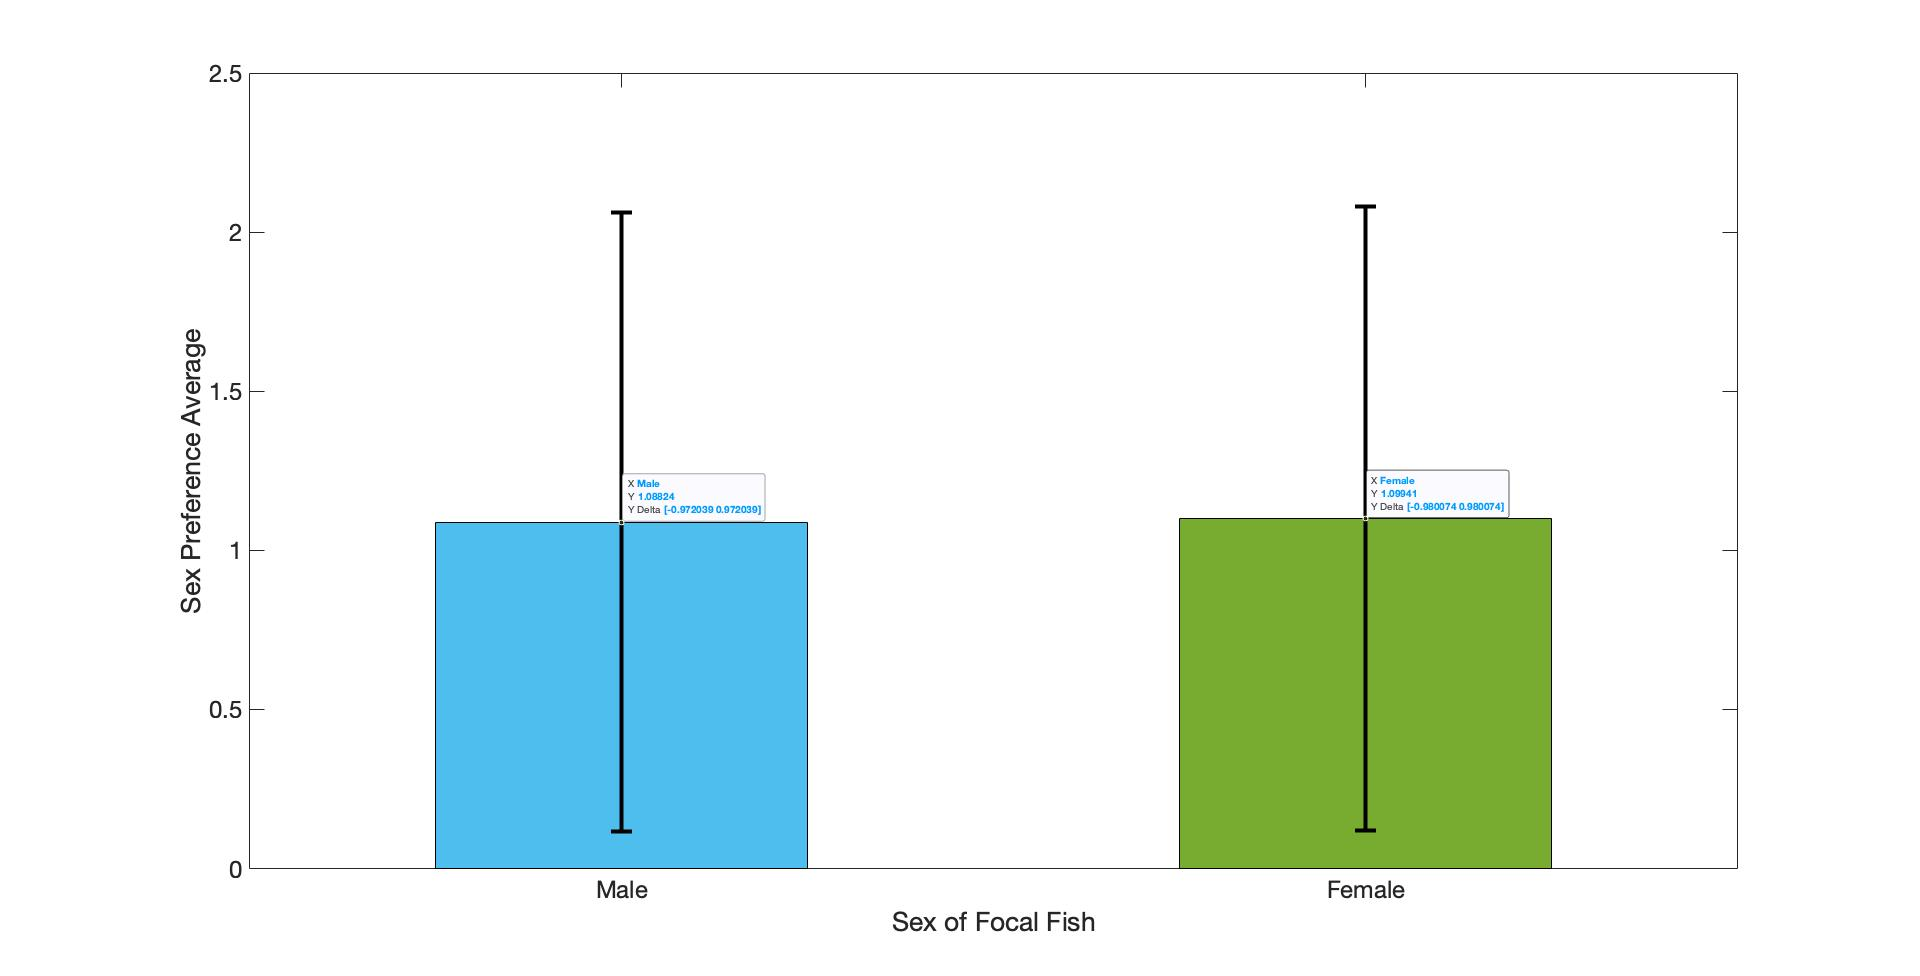
\includegraphics[width=\textwidth]{bars.jpg}
\text{}\\
\fbox{\begin{minipage}{53em}
  \begin{enumerate}
    \item What did you hypothesize about the outcome of this experiment (prior to looking at the data!)?
    \item[] My hypothesis is that the females will prefer showy males and male fishes prefer smaller female fishes.
    \item Do the data provide evidence to support your hypothesis? Explain (in other words, interpret your graph).
    \item[] Male focal fishes prefer larger focal fishes while the female focal fishes prefer showy male fishes.
    \item How does this experiment relate to the concept of sexual selection? (Hint: mate choice based on coloration and morphological features)
    \item[] Males with showy tails are healthier and can possibly give more reproductive success. The showy tail gives a disadvantage to the male from escaping predators, but if the male is able to still maintain a showy tail without getting eaten, they are seen as a “fit” mate for the female (lead to more offspring). Females that are larger can carry more offspring because body size is correlated with number of offspring. So males may choose the larger female because she will lead to more offspring.
  \end{enumerate}
\end{minipage}}
\end{document}